\chapter{\emph{Hamilton-Jacobbi}. Ejemplo}

	
\begin{tikzpicture}
	\fill [left color=red!50, right color=teal!50] (0,0) rectangle (6.5,.1);
	\fill [left color=teal!50, right color=blue!50] (6.5,0) rectangle (11.5,.1);
	\end{tikzpicture}

\vspace{10mm}
\begin{adjustwidth}{50pt}{50pt}
\begin{ejemplo}
Veremos un ejemplo de Hamilton-Jacobbi (H-J) de modo diferente a como lo vimos en el capítulo anterior por que resulta que \textbf{H-J} se puede interpretar como una \textbf{función generadora de una transformación canónica} (TC), lo que resulta muy útil para obtener las ecuaciones del movimiento.

\end{ejemplo}
\end{adjustwidth}
\vspace{5mm}

\section{\emph{Hamilton-Jacobi}. Ejemplo}

\begin{myblock}{Formulación de Hamilton-Jacobi}
\begin{equation}
\label{T27FHJ}
\boldsymbol{
H\left( q_i, \pdv{S}{q_i} \right) + \pdv{S}{t} \ = \ 0 \qquad \qquad \pdv{S}{q_i}\ = \ p_1\ ;\qquad \pdv{S}{t} \ = \ - H
}	
\end{equation}	
\end{myblock}

\textbf{H-J visto como una función generadora de TC}, concretamente de tipo 2, $\boldsymbol {S=F_2}$

En el capítulo \ref{T19FG}, \emph{Funciones generadoras de transformaciones canónicas}, vimos que:

$$F_2(q,P,t)\, : \qquad \qquad \displaystyle \pdv{F_2}{q}=p\, ; \qquad \pdv{F_2}{P}=Q\, ; \qquad \pdv{F_2}{t}=K-H$$

Siendo $K$ el hamiltoniano expresado en las nuevas variables y $H$ el hamiltoniano en las variables antiguas.

Si en vez de llamarla $F_2$ la llamamos $S$, escribiremos,

\begin{equation}
\label{T27StoF}
S=S(q,P,t)\, : \qquad \qquad\pdv{S}{q}=p \, ; \qquad  \pdv{S}{P}=Q\, ; \qquad \pdv{S}{t}=K-H	
\end{equation}

Además de ser $S$ una función de tipo $F_2$, exigimos la condición fuerte de que  sea $\boldsymbol{K=0 \ \to \ \displaystyle \pdv{S}{t}=-H}$ y aplicando las ecuaciones de Hamilton a las nuevas variables, $\displaystyle \dot Q=\pdv{K}{P} \ \wedge \ \dot P=-\pdv{K}{Q}$, al ser $K=0$ obtenemos $\dot Q=0 \ \wedge \ \dot P=0$ con lo que $Q=cte=\beta$ y $P=cte=\alpha$, constantes del movimiento. \textcolor{gris}{Los nombres $\alpha$ y $\beta$ para estas constantes son por razones de notación histórica}. Luego,

\begin{equation}
\label{T27Sqalphat}	
S=S(q,\alpha,t)\, : \qquad \qquad \pdv{S}{q}=p\, ; \qquad \pdv{S}{t}=-H\, ; \qquad \boldsymbol{\pdv{S}{\alpha}=\beta}
\end{equation}

Aparece una nueva pieza, $\ \displaystyle \pdv{S}{\alpha}=\beta \ $, que va a ser muy importante.


Nuestro objetivo es el de siempre, encontrar las ecuaciones del movimiento, es decir, encontrar $\boldsymbol{q(t)}$.

\vspace{10mm}
\subsection{Ejemplo \emph{H-J}}
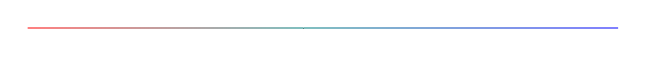
\begin{tikzpicture}
	\fill [left color=red!50, right color=teal!50] (0,0) rectangle (3.5,.01);
	\fill [left color=teal!50, right color=blue!50] (3.5,0) rectangle (7.5,.01);
	\end{tikzpicture}
\vspace{5mm}


\begin{example}

Supongamos un hamiltoniano muy sencillo: $\quad \boldsymbol{ H\ = \ \dfrac 1{2m} \ p^2 \ + \ mgx } $	
\end{example}

\underline{Plan}:

\begin{enumerate}
\item Calcular $S$, llamada \textbf{función principal de Hamilton} o \emph{acción} que depende del punto final y en la que el punto inicial es fijo, tal y como lo interpretábamos en el capítulo anterior.
\item Acudir a la ecuación 	$\ \displaystyle \pdv{S}{\alpha}=\beta \ $  y despejar de ella $q(t)$, la ecuación del movimiento.
\end{enumerate}

\rule{250pt}{0.1pt}

La ecuación de H-J a este hamiltoniano da:
$\ \displaystyle H\left(q_i,\pdv{S}{q_i} \right) + \pdv{S}{t} \quad \longrightarrow \quad \dfrac 1{2m} \left( \pdv{S}{x} \right)^2 + mgx + \pdv{S}{t} = 0$


\begin{enumerate}
\item Vamos a encontrar $S$. Típicamente, $S$ va a ser suma o producto de dos funciones cada una de ellas dependiente de una sola variable, \emph{variables separadas}. Si ello no pudiese ser, recurriríamos a un cambio de variable que lo facilitase.

 En nuestro caso vamos a hacer que $S=f(x)+g(t)$, llevándolo a H-J anterior,
  $\quad \displaystyle \dfrac 1{2m} \left( f'(x) \right)^2 + mgx \ = \ \dot g(t)$
 
 Tenemos una ecuación del tipo  $F(x)=G(t)$ que solo es posible, $\forall x,\ \forall t$ si ocurre que ambas funciones sean la misma constante: $F(x)=G(t)=cte=\alpha\ $ Integrando,
 
 $\triangleright \qquad \dot g = -\alpha \ \to \ g(t)=-\alpha t \ + \cancelto{0}{C}$, tomamos la constante de integración cero porque en las ecuaciones de H-J solo aparecen las derivadas, es una constante aditiva.
 
 $\triangleright \qquad f'=\sqrt{2m(\alpha-mgx)}\ \to \  f(x)=\sqrt{2m}\dfrac{(\alpha -mgx)^{3/2}}{3/2}\dfrac{-1}{mg}=-\dfrac{2\sqrt{2m}}{3mg}(\alpha -mgx)^{3/2}$
 
 Luego, 
 
 \begin{equation}
 \label{T27Sej}
 S\ = \ \textcolor{gris}{f+g} \ = -\boldsymbol \alpha t \ - \ 	\dfrac{2\sqrt{2m}}{3mg}(\boldsymbol \alpha -mgx)^{3/2}
 \end{equation}

\item	$\displaystyle \pdv{S}{\alpha}=\beta \quad \to \quad \beta=-t+\dfrac 2 3 \dfrac{\sqrt{2m}}{mg} \dfrac 3 2 (\alpha-mgx)^{3/2-1}\cdot 1 = -t+\dfrac 1 g \sqrt{\dfrac 2 m} (\alpha-mgx)^{1/2}$

Tenemos que despejar $x \ \to \ \left[ (\beta + t) g \sqrt{\dfrac 2 m} \right]^2=\alpha-mgx \ \to \ x=\dfrac{\alpha}{mg}-\dfrac 1{mg}\left[ (\beta+t)^2 g^2 \dfrac m 2 \right]$

$x=\dfrac{\alpha}{mg}-\dfrac 1 2 g (\beta+t)^2\ $. Interpretemos quienes son $\alpha$ y $\beta$

\vspace{5mm}
------ $\alpha$ es la energía, ya que por la ecuación de H-J, ec. \ref{T27FHJ}, tenemos que $\displaystyle \pdv{S}{t}=-H=-E$ y derivando en la ecuación \ref{T27Sej} tenemos que $\displaystyle \pdv{S}{t}=-\alpha$, por lo que $\alpha=E$

Nuestra función principal del movimiento es, ahora $\ x=\dfrac E{mg}-\dfrac g 2 (\beta+t)^2$

\vspace{5mm}
------ Para determinar $\beta$ procedemos a derivar respecto del tiempo,

$\dot x=-g(\beta + t)=-g\beta -gt$, dimensionalmente $[\dot x]=[gt]=\textit{velocidad}=[g\beta] \ \to \ \  -g\beta=v_0 \ , $

luego $\ \beta=-\dfrac g{v_0}$, por lo que la ecuación de movimiento es, finalmente,

$x=\dfrac E{mg}-\dfrac g 2 \left( - \dfrac{v_0}g + t \right)^2  =
\dfrac E{mg}-\dfrac g 2 \left( \dfrac{v_0^2}{g^2}+t^2-\dfrac{2v_0t}{g} \right)= \dfrac E{mg} -\dfrac 1 2 \dfrac{v_0^2}{g} - \dfrac 1 2 gt^2+v_0t$

Como la energía es constante, $E=\dfrac 1 2 mv^2+mgx=cte=\dfrac 1 2 m v_0^2+mgx_0\ \to \ \dfrac E{mg}=\dfrac{v_0^2}{2g}+x_0$ 

$$\subrayado{ \ \boxed{\  \boldsymbol{ x \ = \ x_0 \ + \ v_0t \ - \ \dfrac 1 2 g t^2 } \ } \ } $$

\vspace{5mm}
En cuanto a la función principal de Hamilton (acción), con $\alpha=E$ se puede expresar, de la ec. \ref{T27Sej}, como
$ \quad \boldsymbol{ S\ = \ - E t \ - \ 	\dfrac{2\sqrt{2m}}{3mg}(E -mgx)^{3/2} } \, . \ \  $
Para que realmente $S=S(t,x)$ y no aparezcan constantes un tanto extrañas $E$ sino que solo aparezcan constantes iniciales $t_0,x_0, m, g$ podemos despejar la $E$ imponiendo que, como $\displaystyle \int_{t_0}^{t_0}\equiv 0$, tendremos que al imponer $s(t_0,x_0)=0$ obtendríamos
$\ 0=-Et_0-\dfrac{2\sqrt{2m}}{3mg}(E-mgx_0)^{3/2}$ y, de aquí, tras pesados pasos despejar la $E$ en función de las constantes iniciales y sustituir en la ecuación de $S(t,x)$


\end{enumerate}










 





















